\subsection{Prijavljivanje klijenta}

Stranica za prijavljivanje klijenta (slika \ref{fig:Login}) ima slične funkcionalnosti kao stranica za registraciju klijenta (slika \ref{fig:SignUp}). Klijent unosi samo svoje korisničko ime i šifru. Ukoliko klijent nema svoj nalog, postoji opcija navigacije ka stranici za prijavljivanje klijenta. Ukoliko je klijent zaboravio svoju šifru, ispod dugmeta \textit{Login}, klikom na opciju \textit{Forgot password?}, klijentu se automatski šalje mejl na prijavljenu email adresu sa instrukcijama za oporavak šifre. 

\begin{figure}[H]
	\begin{center}
		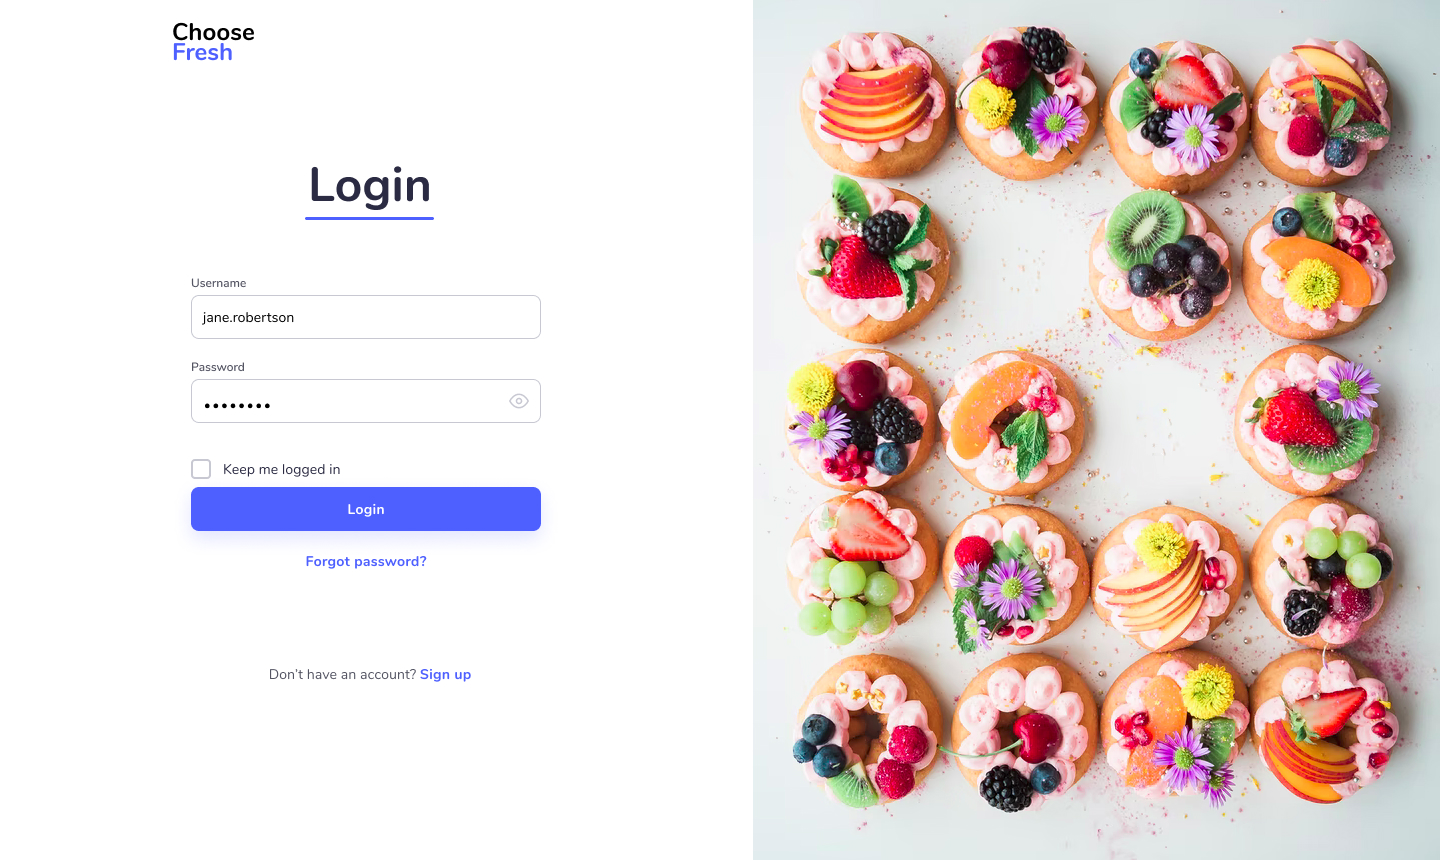
\includegraphics[width=\textwidth]{UI/Login.jpg}
    		\caption{Stranica za prijavljivanje klijenta}
    \label{fig:Login}
    \end{center}
\end{figure}

Ako klijent unese pogrešne podatke za prijavljivanje na sistem, prikazuje se stranica \ref{fig:WrongInput}. U slučaju da klijent više puta pokušava da se prijavi na sistem sa pogrešnim podacima, pojavljuje se prozor koji obaveštava klijenta da može pokušati ponovo tek nakon 1h (slika \ref{fig:BruteForceAttack}).
\begin{figure}[H]
	\begin{center}
		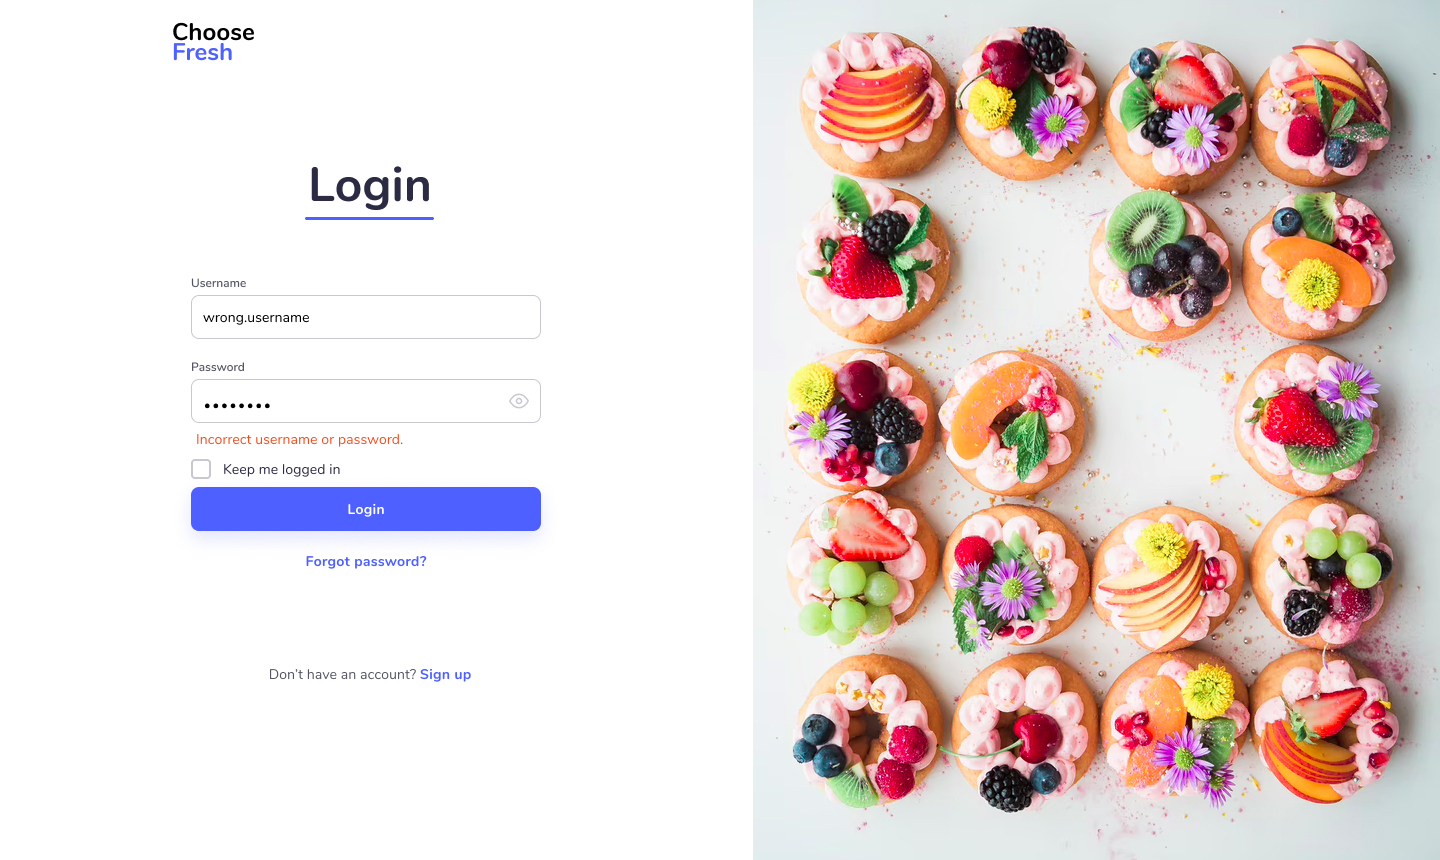
\includegraphics[width=\textwidth]{UI/WrongInput.jpg}
    		\caption{Stranica za prijavljivanje klijenta ako je uneo pogrešne podatke}
    \label{fig:WrongInput}
    \end{center}
\end{figure}

\begin{figure}[H]
	\begin{center}
		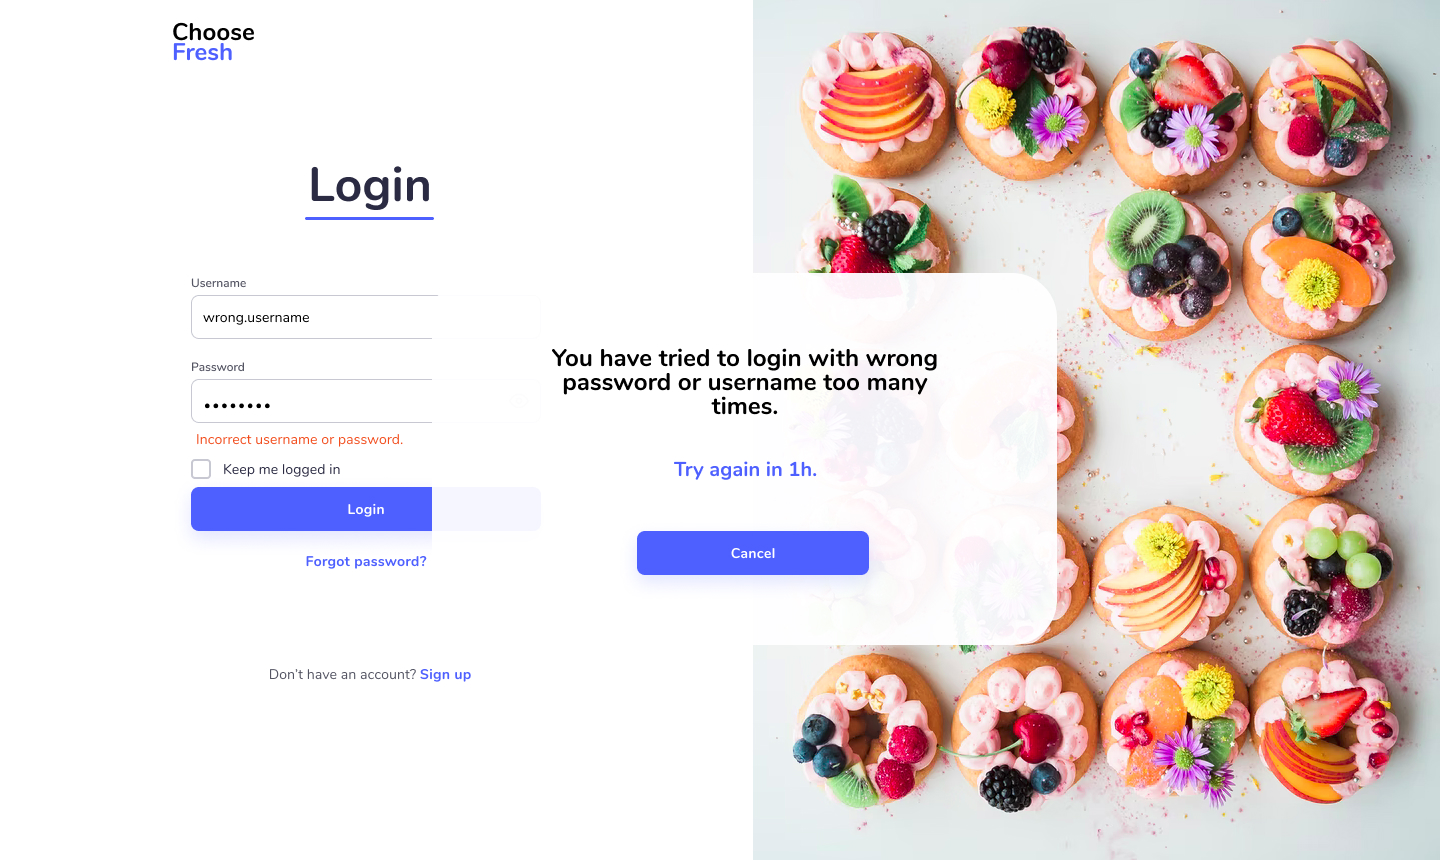
\includegraphics[width=\textwidth]{UI/BruteForceAttack.jpg}
    		\caption{Stranica za prijavljivanje klijenta ukoliko je neuspešno prijavljivanje nakon više pokušaja}
    \label{fig:BruteForceAttack}
    \end{center}
\end{figure}
